\tikzset{every picture/.style={line width=0.75pt}} %set default line width to 0.75pt        

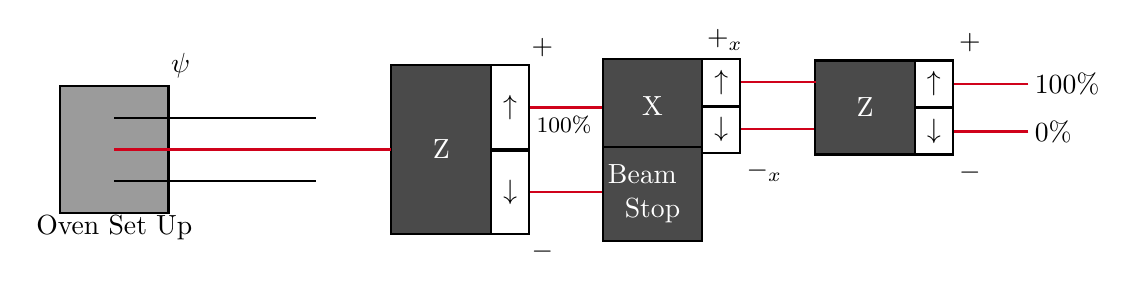
\begin{tikzpicture}[x=0.75pt,y=0.75pt,yscale=-.8,xscale=.8]
%uncomment if require: \path (0,375); %set diagram left start at 0, and has height of 375

%Shape: Rectangle [id:dp14421103605944618] 
\draw  [fill={rgb, 255:red, 155; green, 155; blue, 155 }  ,fill opacity=1 ] (13.01,128) -- (78.24,128) -- (78.24,204) -- (13.01,204) -- cycle ;
%Straight Lines [id:da6727148484422872] 
\draw [color={rgb, 255:red, 208; green, 2; blue, 27 }  ,draw opacity=1 ]   (167.01,166) -- (45.63,166) ;
%Shape: Rectangle [id:dp31052784363324215] 
\draw  [fill={rgb, 255:red, 74; green, 74; blue, 74 }  ,fill opacity=1 ] (212.51,115.36) -- (272.59,115.36) -- (272.59,216.64) -- (212.51,216.64) -- cycle ;
%Straight Lines [id:da9714115391207371] 
\draw    (167.01,147) -- (45.63,147) ;
%Straight Lines [id:da9565511475124852] 
\draw    (167.01,185) -- (45.63,185) ;
%Straight Lines [id:da5775689584288694] 
\draw [color={rgb, 255:red, 208; green, 2; blue, 27 }  ,draw opacity=1 ]   (212.01,166) -- (167.01,166) ;
%Shape: Rectangle [id:dp34780699384586333] 
\draw  [fill={rgb, 255:red, 255; green, 255; blue, 255 }  ,fill opacity=1 ] (272.59,167) -- (295.4,167) -- (295.4,216.64) -- (272.59,216.64) -- cycle ;
%Shape: Rectangle [id:dp9674012952324293] 
\draw  [fill={rgb, 255:red, 255; green, 255; blue, 255 }  ,fill opacity=1 ] (272.59,115.36) -- (295.4,115.36) -- (295.4,166) -- (272.59,166) -- cycle ;
%Straight Lines [id:da8039050506004896] 
\draw [color={rgb, 255:red, 208; green, 2; blue, 27 }  ,draw opacity=1 ]   (341.01,140.68) -- (296.01,140.68) ;
%Straight Lines [id:da5371523365899473] 
\draw [color={rgb, 255:red, 208; green, 2; blue, 27 }  ,draw opacity=1 ]   (341.01,191.82) -- (296.01,191.82) ;
%Shape: Rectangle [id:dp5066877735662358] 
\draw  [fill={rgb, 255:red, 74; green, 74; blue, 74 }  ,fill opacity=1 ] (339.68,111.36) -- (399.77,111.36) -- (399.77,168) -- (339.68,168) -- cycle ;
%Shape: Rectangle [id:dp7068517018359358] 
\draw  [fill={rgb, 255:red, 255; green, 255; blue, 255 }  ,fill opacity=1 ] (399.77,140.24) -- (422.58,140.24) -- (422.58,168) -- (399.77,168) -- cycle ;
%Shape: Rectangle [id:dp5547396655118183] 
\draw  [fill={rgb, 255:red, 255; green, 255; blue, 255 }  ,fill opacity=1 ] (399.77,111.36) -- (422.58,111.36) -- (422.58,139.68) -- (399.77,139.68) -- cycle ;

%Straight Lines [id:da995628624290608] 
\draw [color={rgb, 255:red, 208; green, 2; blue, 27 }  ,draw opacity=1 ]   (468.19,153.82) -- (423.19,153.82) ;
%Shape: Rectangle [id:dp5083037352636465] 
\draw  [fill={rgb, 255:red, 74; green, 74; blue, 74 }  ,fill opacity=1 ] (339.68,164.36) -- (399.77,164.36) -- (399.77,221) -- (339.68,221) -- cycle ;
%Shape: Rectangle [id:dp3008323325045591] 
\draw  [fill={rgb, 255:red, 74; green, 74; blue, 74 }  ,fill opacity=1 ] (467.68,112.36) -- (527.77,112.36) -- (527.77,169) -- (467.68,169) -- cycle ;
%Shape: Rectangle [id:dp24796764616598033] 
\draw  [fill={rgb, 255:red, 255; green, 255; blue, 255 }  ,fill opacity=1 ] (527.77,141.24) -- (550.58,141.24) -- (550.58,169) -- (527.77,169) -- cycle ;
%Shape: Rectangle [id:dp4270203138981403] 
\draw  [fill={rgb, 255:red, 255; green, 255; blue, 255 }  ,fill opacity=1 ] (527.77,112.36) -- (550.58,112.36) -- (550.58,140.68) -- (527.77,140.68) -- cycle ;

%Straight Lines [id:da8067196861586373] 
\draw [color={rgb, 255:red, 208; green, 2; blue, 27 }  ,draw opacity=1 ]   (596.17,126.52) -- (551.17,126.52) ;
%Straight Lines [id:da7594531119094955] 
\draw [color={rgb, 255:red, 208; green, 2; blue, 27 }  ,draw opacity=1 ]   (596.17,155.12) -- (551.17,155.12) ;
%Straight Lines [id:da2036670384719227] 
\draw [color={rgb, 255:red, 208; green, 2; blue, 27 }  ,draw opacity=1 ]   (468.17,125.52) -- (423.17,125.52) ;

% Text Node
\draw (45.63,204) node [anchor=north] [inner sep=0.75pt]   [align=left] {\begin{minipage}[lt]{61.13pt}\setlength\topsep{0pt}
\begin{center}
Oven Set Up
\end{center}

\end{minipage}};
% Text Node
\draw (242.55,166) node  [color={rgb, 255:red, 255; green, 255; blue, 255 }  ,opacity=1 ] [align=left] {Z};
% Text Node
\draw (284,140.68) node    {$\uparrow $};
% Text Node
\draw (284,191.82) node  [rotate=-180]  {$\uparrow $};
% Text Node
\draw (77.91,124.6) node [anchor=south west] [inner sep=0.75pt]    {$\ket{\psi }$};
% Text Node
\draw (295.07,111.96) node [anchor=south west] [inner sep=0.75pt]    {$\ket{+}$};
% Text Node
\draw (295.14,220.04) node [anchor=north west][inner sep=0.75pt]    {$\ket{-}$};
% Text Node
\draw (400.77,107.96) node [anchor=south west] [inner sep=0.75pt]    {$\ket{+}_{x}$};
% Text Node
\draw (369.73,139.68) node  [color={rgb, 255:red, 255; green, 255; blue, 255 }  ,opacity=1 ] [align=left] {X};
% Text Node
\draw (411.17,125.52) node    {$\uparrow $};
% Text Node
\draw (411.17,154.12) node  [rotate=-180]  {$\uparrow $};
% Text Node
\draw (598.17,126.52) node [anchor=west] [inner sep=0.75pt]    {$100\%$};
% Text Node
\draw (539.17,155.12) node  [rotate=-180]  {$\uparrow $};
% Text Node
\draw (539.17,126.52) node    {$\uparrow $};
% Text Node
\draw (497.73,140.68) node  [color={rgb, 255:red, 255; green, 255; blue, 255 }  ,opacity=1 ] [align=left] {Z};
% Text Node
\draw (598.17,155.12) node [anchor=west] [inner sep=0.75pt]    {$0\%$};
% Text Node
\draw (552.58,108.96) node [anchor=south west] [inner sep=0.75pt]    {$\ket{+}$};
% Text Node
\draw (552.58,172.4) node [anchor=north west][inner sep=0.75pt]    {$\ket{-}$};
% Text Node
\draw (369.73,192.68) node  [color={rgb, 255:red, 255; green, 255; blue, 255 }  ,opacity=1 ] [align=left] {\begin{minipage}[lt]{32.21pt}\setlength\topsep{0pt}
Beam 
\begin{center}
Stop
\end{center}

\end{minipage}};
% Text Node
\draw (298.01,144.08) node [anchor=north west][inner sep=0.75pt]    {\footnotesize $100\%$};
% Text Node
\draw (424.58,171.4) node [anchor=north west][inner sep=0.75pt]    {$\ket{-}_{x}$};


\end{tikzpicture}
